\documentclass[tikz, border=20pt]{standalone}
\usepackage[utf8]{inputenc}
\usepackage[T5]{fontenc}
\usepackage{lmodern}
\usepackage{xcolor}
\usepackage{graphicx}
\usetikzlibrary{positioning, calc, arrows}

\begin{document}
\begin{tikzpicture}[
  >=stealth,
  font=\sffamily,
  % Định dạng 4 cột chuẩn xác, chiều cao và độ rộng đồng nhất tuyệt đối
  tierCard/.style={
    draw=black,
    dashed,
    line width=1.4pt,
    fill=white,
    rounded corners=6pt,
    inner sep=8pt,
    text width=6.2cm,
    minimum height=14.0cm,
    align=center
  },
  % Nhãn trên mũi tên
  tagText/.style={
    font=\small\bfseries,
    fill=white,
    inner sep=3.5pt,
    rounded corners=3pt,
    draw=black!50,
    line width=0.7pt,
    text=black
  },
  arrowThick/.style={
    ->,
    line width=2.0pt,
    draw=black
  },
  biArrowThick/.style={
    <->,
    line width=2.0pt,
    draw=black
  }
]

% ==================== 4 CỘT KIẾN TRÚC ĐỒNG NHẤT TUYỆT ĐỐI (ANCHOR=NORTH) ====================

% CỘT 1: TẦNG ĐEO
\node[tierCard, anchor=north] (col1) at (-12.6, 6.0) {
  {\bfseries\Large TẦNG 1: TẦNG ĐEO}\\[3pt]
  {\footnotesize\color{black!70} (Wearable Physical Tier)}\\[10pt]
  
  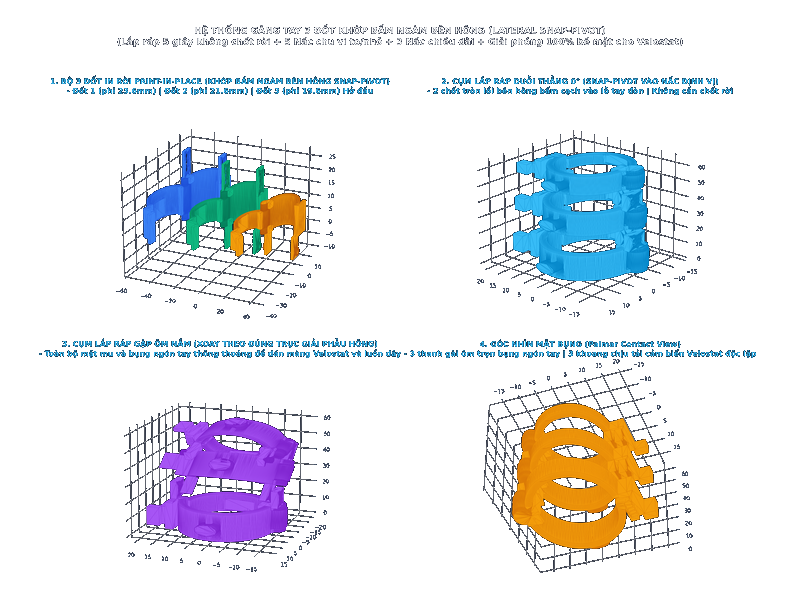
\includegraphics[width=5.6cm, height=3.2cm, keepaspectratio]{assets/splint_3d_transparent.png}\\[4pt]
  {\bfseries\normalsize Khung nẹp 3 ngón in 3D}\\[2pt]
  {\footnotesize Ngàm xoay 2 bản lề tháo mở 1 tay}\\[10pt]
  
  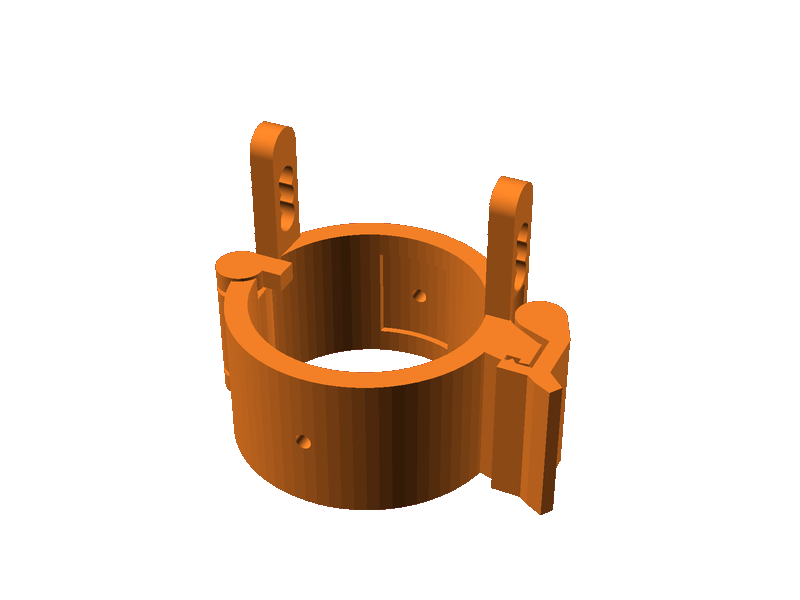
\includegraphics[width=4.8cm, height=2.2cm, keepaspectratio]{assets/mech9_transparent.png}\\[4pt]
  {\bfseries\normalsize Cảm biến lực \& góc uốn}\\[16pt]
  
  {\bfseries\large Chức năng tầng đeo}\\[8pt]
  \parbox{5.8cm}{\centering\normalsize
    $\bullet$ 16 Ô Velostat vi sai lòng--mu bàn tay\\[5pt]
    $\bullet$ 3 Cảm biến uốn Flex đo góc khớp ngón\\[5pt]
    $\bullet$ Đệm bọt EVA phân bổ đều áp lực ngón\\[5pt]
    $\bullet$ Thu nhận nỗ lực vận động cơ năng
  }
};

% CỘT 2: TẦNG THU THẬP & DSP
\node[tierCard, anchor=north, right=72pt of col1] (col2) {
  {\bfseries\Large TẦNG 2: THU THẬP \& DSP}\\[3pt]
  {\footnotesize\color{black!70} (Sensing \& DSP Tier)}\\[10pt]
  
  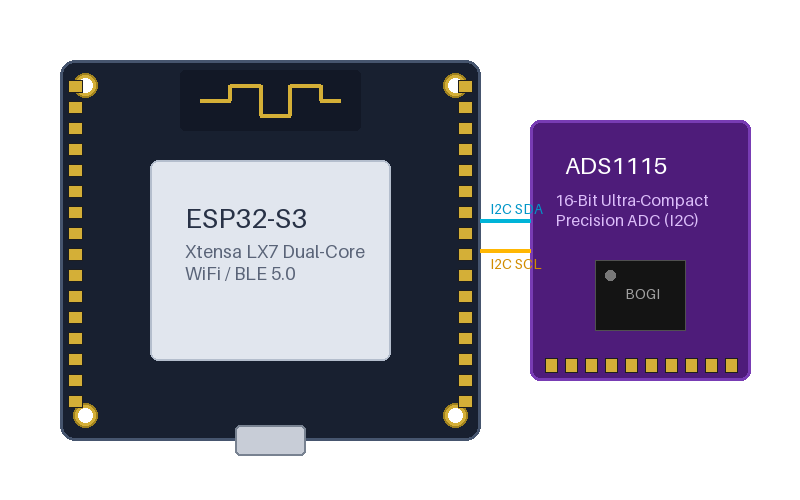
\includegraphics[width=5.4cm, height=3.0cm, keepaspectratio]{assets/controller_ads_board.png}\\[4pt]
  {\bfseries\normalsize ESP32-S3 + ADS1115 (16-bit)}\\[2pt]
  {\footnotesize 2 MUX CD74HC4067 (21 kênh $\ge$15Hz)}\\[50pt]
  
  {\bfseries\large Xử lý tín hiệu số (DSP)}\\[8pt]
  \parbox{5.8cm}{\centering\normalsize
    $\bullet$ Bám nền động khử trôi tĩnh Velostat\\[5pt]
    $\bullet$ Ngưỡng thích nghi 180 mV vi sai\\[5pt]
    $\bullet$ Trích xuất bộ ba chỉ số EI -- GAP -- RAL\\[5pt]
    $\bullet$ Thuật toán AAN 3 pha trợ lực theo nhu cầu
  }
};

% CỘT 3: TẦNG TRỢ LỰC CƠ HỌC
\node[tierCard, anchor=north, right=72pt of col2] (col3) {
  {\bfseries\Large TẦNG 3: TRỢ LỰC}\\[3pt]
  {\footnotesize\color{black!70} (Actuation Tier)}\\[10pt]
  
  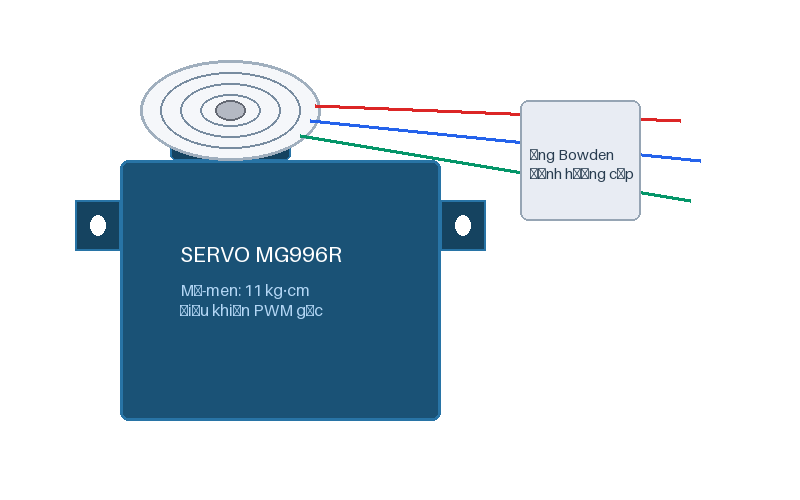
\includegraphics[width=5.4cm, height=3.0cm, keepaspectratio]{assets/servo_spool_assembly.png}\\[4pt]
  {\bfseries\normalsize 3 Servo MG996R \& Tang cáp}\\[2pt]
  {\footnotesize Lực kéo 11 kg$\cdot$cm chủ động 3 ngón}\\[50pt]
  
  {\bfseries\large Truyền động cáp Bowden}\\[8pt]
  \parbox{5.8cm}{\centering\normalsize
    $\bullet$ Cáp Dyneema trượt trong ống Teflon\\[5pt]
    $\bullet$ Kéo gập chủ động hỗ trợ nỗ lực người bệnh\\[5pt]
    $\bullet$ Servo chủ động nhả cáp khi người bệnh duỗi\\[5pt]
    $\bullet$ Nẹp đàn hồi hồi vị đẩy mở ngón an toàn
  }
};

% CỘT 4: TẦNG THỊ GIÁC 3D & TÁC VỤ
\node[tierCard, anchor=north, right=72pt of col3] (col4) {
  {\bfseries\Large TẦNG 4: THỊ GIÁC 3D}\\[3pt]
  {\footnotesize\color{black!70} (Vision Pre-Actuation Tier)}\\[10pt]
  
  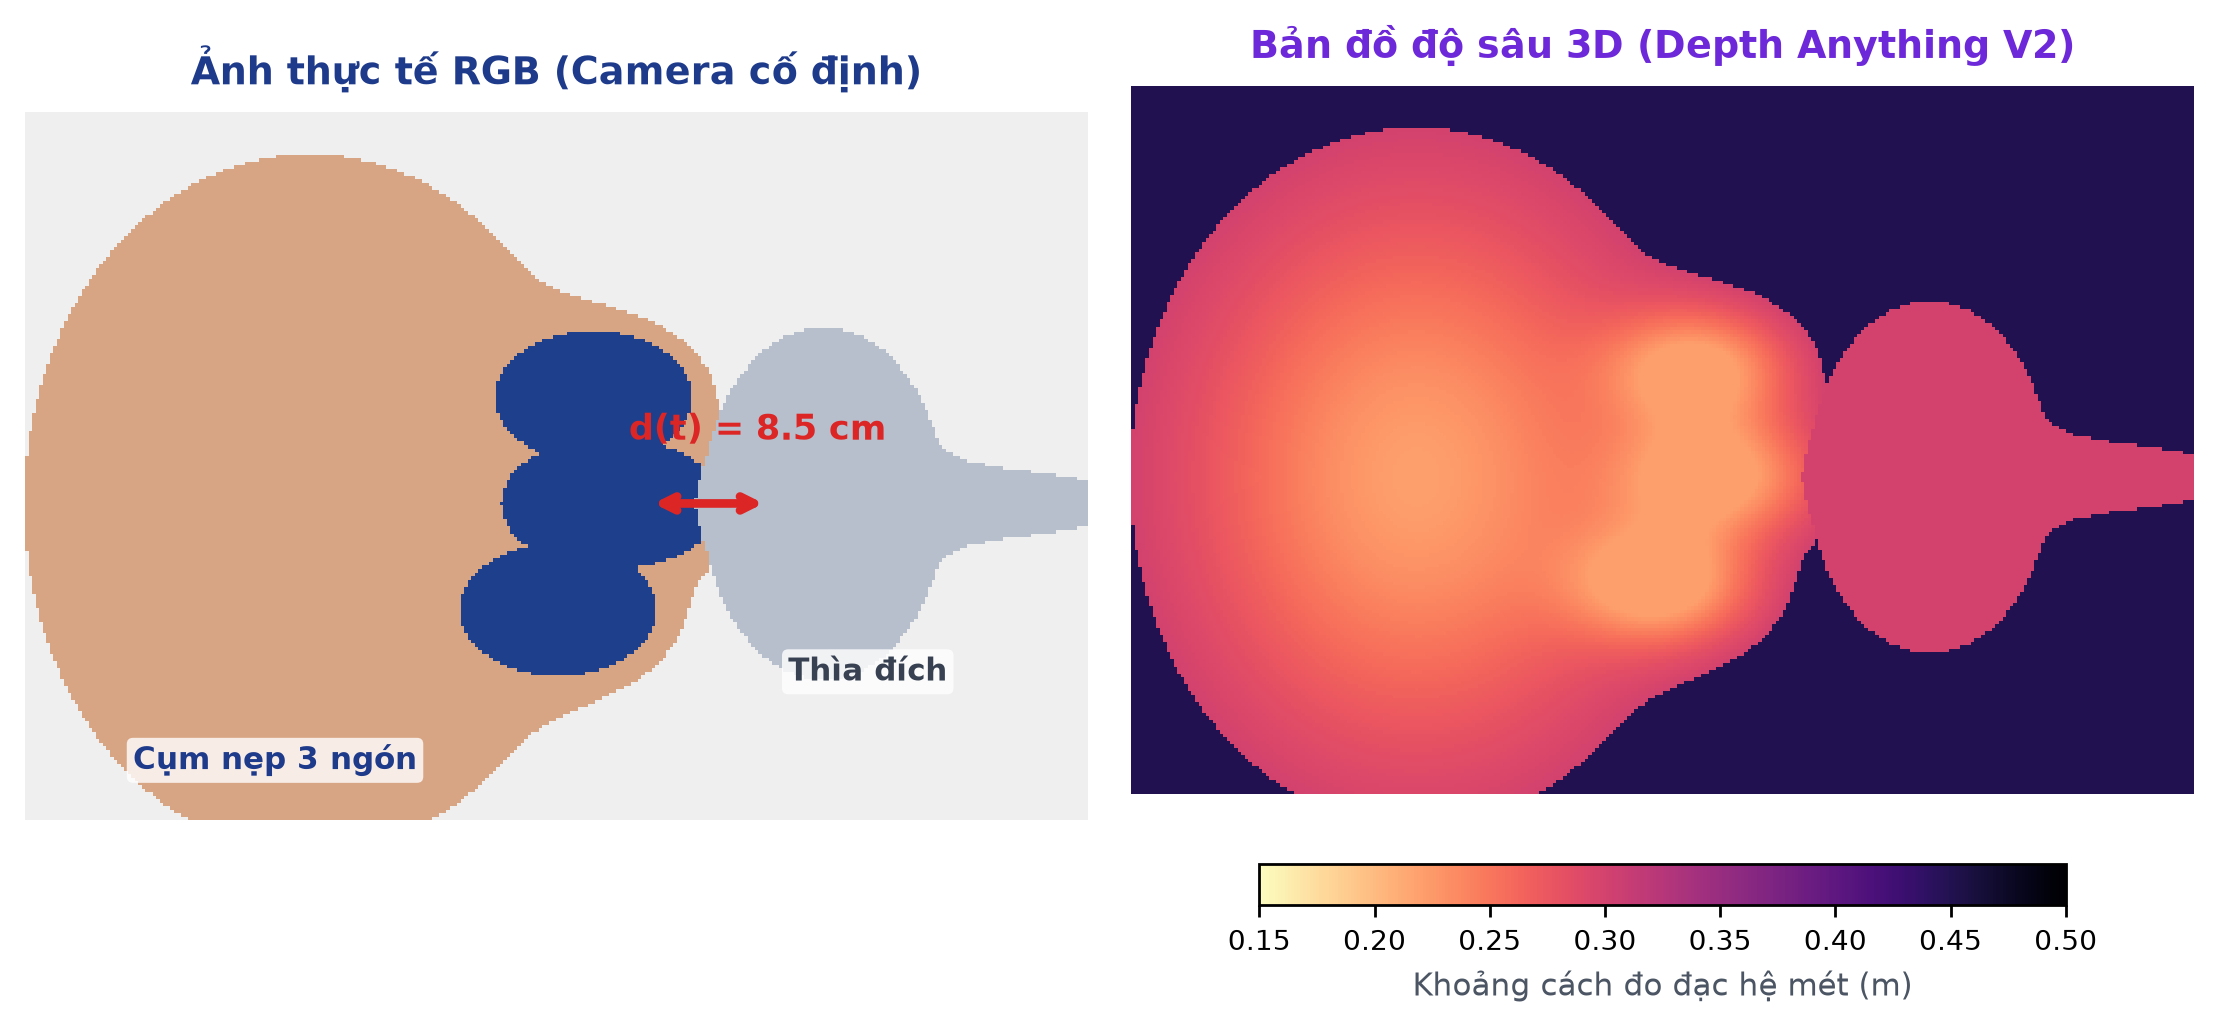
\includegraphics[width=5.6cm, height=3.0cm, keepaspectratio]{assets/depth_anything_scene.png}\\[4pt]
  {\bfseries\normalsize Depth Anything V2 (3D)}\\[2pt]
  {\footnotesize Camera RGB + Bản đồ độ sâu hệ mét}\\[50pt]
  
  {\bfseries\large Orange Pi 5 Pro (NPU)}\\[8pt]
  \parbox{5.8cm}{\centering\normalsize
    $\bullet$ Ước lượng cự ly 3D tay -- thìa $d(t)$\\[5pt]
    $\bullet$ Dự báo thời gian tiếp xúc TTC đón trước\\[5pt]
    $\bullet$ Điều chỉnh khẩu độ ngón trước khi kẹp\\[5pt]
    $\bullet$ Phản hồi thị giác tiến trình tập luyện
  }
};

% ==================== MŨI TÊN KẾT NỐI NGANG THẲNG TẮP ====================

% Tầng 1 -> Tầng 2
\draw[arrowThick] ($(col1.north east)!0.45!(col1.south east)$) -- 
  node[tagText, above=3pt] {Tín hiệu 21 kênh} 
  node[tagText, below=3pt] {Áp lực vi sai \& Góc} 
  ($(col2.north west)!0.45!(col2.south west)$);

% Tầng 2 -> Tầng 3
\draw[arrowThick] ($(col2.north east)!0.45!(col2.south east)$) -- 
  node[tagText, above=3pt] {Lệnh servo AAN} 
  node[tagText, below=3pt] {Kéo gập / Nhả duỗi} 
  ($(col3.north west)!0.45!(col3.south west)$);

% Tầng 4 <-> Tầng 2/3: Trao đổi dữ liệu đón trước
\draw[biArrowThick] ($(col4.north west)!0.45!(col4.south west)$) -- 
  node[tagText, above=3pt] {Cự ly 3D $d(t)$} 
  node[tagText, below=3pt] {TTC đón trước} 
  ($(col3.north east)!0.45!(col3.south east)$);

% ==================== VÒNG PHẢN HỒI CƠ HỌC (UỐN CHỮ U ĐỒNG DẠNG, VUÔNG GÓC 90 ĐỘ TUYỆT ĐỐI) ====================
\draw[arrowThick, dashed] (col3.south) -- ++(0, -1.2cm) 
  -- ($(col1.south) + (0, -1.2cm)$) 
  node[tagText, midway, fill=white, inner sep=4pt] {Vòng cơ học: Cáp Bowden kéo trợ lực gập ngón / Nhả duỗi mở khẩu độ} 
  -- (col1.south);

\end{tikzpicture}
\end{document}
